\documentclass[12pt]{article}
\usepackage[utf8]{inputenc}
\usepackage{hyperref}
\usepackage[a4paper]{geometry}
\usepackage{listings}
\usepackage{fancyvrb}
\usepackage{tikz}
\usetikzlibrary{trees,positioning}

\begin{document}

\begin{center}
	{\Large Training Project Laboratory:} \\
	{\bf \Huge C compiler} \\[3mm]
	{\bf György Kurucz} \\
	{Budapest University of Technology and Economics} \\
	{gyuri@sch.bme.hu} \\[10mm]
\end{center}

\hfil {\bf \Large Abstract} \hfil \\[1mm]
The goal of the project was to implement a C11~\cite{c11} compiler with a small
feature set. A lexical analyzer, parser, syntax tree, and a code generator had
to be implemented to accomplish this goal. The program takes in a source text
file, and outputs \texttt{x86-64} assembly. Enough language features were
implemented to make Turing-complete programs. (We demonstrate this using a
Brainfuck interpreter.) Additional language features, such as basic type
checking, and scopes were also implemented.

\section{Introduction}
While the C language can appear quite dated compared to some newer languages,
it still underpins most of our modern infrastructure. Even if you don't use it
directly, chances are, the compiler/interpreter for your favorite language was
written in C. The kernel your computer is running has almost certainly been
written in C.

In this paper, I will showcase the components of the compiler in the order they
process the source code:
\begin{itemize}
	\item The lexical analyzer turns raw text into tokens.
	\item The parser turns tokens into an abstract syntax tree.
	\item The abstract syntax tree itself.
	\item The code generator traverses the syntax tree, and outputs assembly.
\end{itemize}

The code can be found at \url{https://git.sch.bme.hu/gyuri/c_compiler}. (This
version of the paper corresponds to the \texttt{@VCS_TAG@} revision.)

\section{Lexical analysis}
Because writing lexical analyzers (lexer for short) is a common problem, lexer
generators exist that create the lexer from a compact domain specific language
used to represent the lexical rules. I used \texttt{flex}~\cite{flex} to
generate my lexer.

Fortunately, the lexical rules for C are quite simple. (The preprocessor is not
implemented here, the lexer expects a preprocessed C source.)  We need to
recognize comments, string literals, numeric literals, keywords, identifiers,
and operators. Comments and whitespace are ignored (we simply don't emit any
tokens). (Whitespace is only used to separate otherwise ambiguous tokens.)

As an example, I will show how the lexical rule for identifiers is implemented.
First, we look at what the standard says about identifiers:
``An identifier is a sequence of nondigit characters (including the underscore
\texttt{\_}, the lowercase and uppercase Latin letters, and other characters)
and digits''

The standars also says that identifiers must not start with a digit. Based on
these, we can describe identifiers with the following regular expression:
\begin{center}
\begin{BVerbatim}
{nondigit}({nondigit}|{digit})*
\end{BVerbatim}
\end{center}

Not all rules are so complex, for instance keywords or operators simply need to
recognize themselves:
\begin{center}
\begin{BVerbatim}
_Bool return U_BOOL;
"++" return INCR;
\end{BVerbatim}
\end{center}

For all the rules, see \texttt{src/c.l} in the source code.

\section{Parsing}
Similarly to the lexer, the parser is also usually generated. The parser
generator \texttt{bison}~\cite{bison} is employed for this task. I stick mostly
to the original \texttt{yacc} features, with only a few \texttt{bison}
extensions. Rules are written as a BNF-like grammar, with C snippets used as
actions when a certain rule is recognized by the parser. I use these actions to
directly construct the abstract syntax tree.

There are some very simple rules, that only recognize single tokens. For
instance, this rule recognizes all unary operators.
\begin{center}
\begin{BVerbatim}
unary_operator : AND { $$ = AST_UNARY_REF; }
	       | STAR { $$ = AST_UNARY_DEREF; }
	       | PLUS { $$ = AST_UNARY_PLUS; }
	       | MINUS { $$ = AST_UNARY_MINUS; }
	       | NOT { $$ = AST_UNARY_NOT; }
	       | NOTB { $$ = AST_UNARY_NOTB; }
	       ;
\end{BVerbatim}
\end{center}

These are then used in higher level rules. Here, we recognize unary
expressions. Note, that increment and decrement operators are handled
separately, since for these, there is no direct correspondence between a token,
and the operation it denotes. A \texttt{++} token can denote either a pre, or a
post increment operator. This grammar rule only recognizes prefix operators.
(The postfix variants are handled by a different rule.)
\begin{center}
\begin{BVerbatim}
unary_expression : postfix_expression { $$ = $1; }
		 | INCR unary_expression { $$ = ast_unary($2, AST_PRE_INCR); }
		 | DECR unary_expression { $$ = ast_unary($2, AST_PRE_DECR); }
		 | unary_operator cast_expression { $$ = ast_unary($2, $1); }
		 ;
\end{BVerbatim}
\end{center}

At the top, we arrive at the \texttt{translation\_unit} rule. It simply says
that a C file is a list of function definitions, and declarations.
\begin{center}
\begin{BVerbatim}
translation_unit : external_declaration { $$ = ast_translation_unit($1); }
		 | translation_unit external_declaration {
	vec_append(&($1)->translation_unit, &($2)); $$ = $1; }
		 ;
external_declaration : function_definition { $$ = $1; }
		     | declaration { $$ = $1; }
		     ;
\end{BVerbatim}
\end{center}
(Note that the \verb|{ $$ = $1; }| action is not needed, as this would be the
default action anyway. I simply included it for clarity.)

\subsection{Limitations}
I did not implement type definitions. As the C grammar is \emph{almost}
context-free, this would \emph{almost} make parsing as easy as I described
above. Unfortunately, typedefs make the grammar ambiguous. Consider the
following example:
\begin{center}
\begin{BVerbatim}
a * b;
\end{BVerbatim}
\end{center}

Whether this is a multiplication experssion, or a declaration depends on
whether \texttt{a} is a typedef name.

To make matters worse, typedef names are also have to adhere to scoping:
\begin{center}
\begin{BVerbatim}
typedef int T;
int x;
void f() {
	T y = 1; // T is a type
	if (1) {
		int T;
		T * x; // T is a variable, so this is multiplication
	}
	T * x; // T is a type again, so this declares a variable named x
}
\end{BVerbatim}
\end{center}

For an in-depth discussion about \emph{correct} C parsing, see
\cite{c11_parsing}.

\section{The abstract syntax tree}

\begin{figure}
\centering
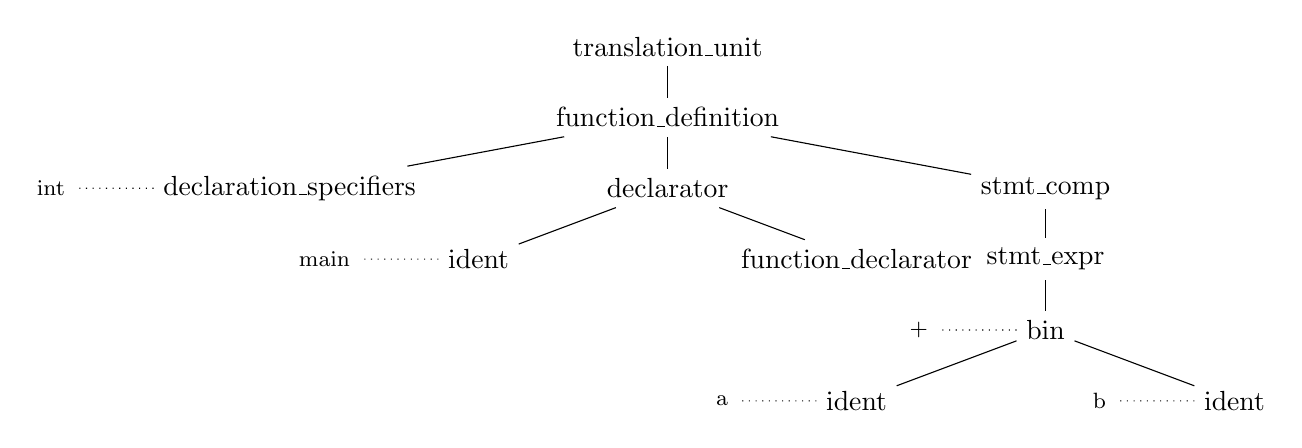
\begin{tikzpicture}[ scale=0.6, level 2/.style={sibling distance=80mm} ]
	\node (a) {translation\_unit}
	child {
		node (b) {function\_definition}
		child {
			node (c) {declaration\_specifiers}
		}
		child {
			node (d) {declarator}
			child {
				node (e) {ident}
			}
			child {
				node (f) {function\_declarator}
			}
		}
		child {
			node (g) {stmt\_comp}
			child {
				node (h) {stmt\_expr}
				child {
					node (i) {bin}
					child { node (j) {ident} }
					child { node (k) {ident} }
				}
			}
		}
	};
	\begin{scope}[every node/.style={font=\footnotesize}]
		\node[left=of c] (nc) {int};
		\node[left=of e] (ne) {main};
		\node[left=of i] (ni) {+};
		\node[left=of j] (nj) {a};
		\node[left=of k] (nk) {b};
		% \node[right=of d] (nd) {\{T.v${}$F.v$^{*}$T.v\}};
		% \node[right=of i] (ni) {\{F.v${}$2\}};
		% \node[left=of b] (nb) {\{F.v${}$5\}};
		% \node[left=of e] (ne) {\{T.v${}$F.v\}};
		% \node[left=of f] (nf) {\{F.v${}$8\}};
		\foreach \i in {c,e,i,j,k}
			\draw[dotted] (\i) -- (n\i);
	\end{scope}
\end{tikzpicture}
\caption{An abstract syntax tree}
\label{fig:ast}
\end{figure}

The syntax tree is made up of polymorphic nodes. The leaves of the tree are
usually identifiers or literals. (We can also have for example an empty
expression statement, but this is unusual.)

Let's look at the following program.~\footnote{This program is only
syntactically correct. \texttt{a} and \texttt{b} are undeclared identifiers.}
(See Figure~\ref{fig:ast} for the syntax tree.)
\begin{center}
\begin{BVerbatim}
int main() { a + b; }
\end{BVerbatim}
\end{center}

At the top of every program, we find the translation unit. Inside this, we have
declarations, and function definitions. Inside the function definitions, we can
find statements, and possibly more declarations. There are many kinds of
statements, an expression statement is simply an expression that is evaluated
only for it's side effects (the resulting value of the expression is simply
thrown away).

\section{Code generation}
While most compilers use some sort of intermediate representation when
generating machine code, C is so simple, that we can generate the code with a
single traversal of the syntax tree. (Note that we don't do any optimization.)

My implementation emits \texttt{x86-64} assembly, and I will also use that here
to show some examples of generated code.

\subsection{State}
The code generator uses the following state during traversal:
\begin{itemize}
	\item The stack pointer (used to allocate new variables on the stack,
		and to set the actual stack pointer when calling a function.)
	\item The current stack of scopes.
	\item The declared variables (inside each scope).
	\item The string literals used in the program.
\end{itemize}

\subsection{Values}
Each expression has a value it evaluates to. We represent such a value with a
handle, with the following attributes:
\begin{itemize}
	\item It's type.
	\item Whether it is an lvalue.
	\item A location on the stack.
	\item The number of times this value on the stack has to be
		dereferenced to get to the actual value.
\end{itemize}

We make an important simplifying assumption here: that any value can be stored
fully in a processor register. This is generally not true, because for instance
C allows struct values: \verb|(struct a){ 0 }|.

\newcommand{\compexample}[2]{
	\begin{center}
	\fbox {
		\begin{minipage}{0.5\textwidth}
		\hfil {\bf Example:} For the C code \hfil

		\begin{center} {\tt #1} \end{center}

		\hfil the generated code is: \hfil

		\vspace{1mm}

		{\tt #2}
		\end{minipage}
	}
	\end{center}
}

\subsection{Expressions}
The code generator for expressions (see \texttt{cg\_gen\_expr} in \texttt{src/cg.c})
does two things: generates code to evaluate the expression, and returns a
handle for the resulting value.

If the expression is a literal, this is very simple: emit code for moving the
literal onto the stack, and return the stack position as a value handle.

\compexample{4}{
mov rax, 4 \\
mov dword [rbp-8], eax ; store
}

If the expression is an identifier, we look up the corresponding variable in
our current stack of scopes, and return its value handle.

If the expression is a unary or binary operator, the generally following scheme is followed:
\begin{enumerate}
	\item Call the expression code generator for each operand.
	\item Emit code for performing the operation.
	\item Emit code for moving the result onto the stack, and return the
		value handle.
\end{enumerate}

\compexample{
int a; \\
++a;
}{
; alloced `a` on stack at -8 \\
xor rax, rax \\
mov eax, dword [rbp-8] ; read \\
add rax, 1 \\
mov dword [rbp-8], eax ; store
}

Function calls are somewhat more involved because of the ABI, but conceptually
basically the same: generate code for all operands, emit code for call, return
value handle for result.

\compexample{
int b = f(1);
}{
; alloced `b` on stack at -8 \\
mov rax, 1 \\
mov dword [rbp-16], eax ; store \\
xor rax, rax \\
mov eax, dword [rbp-16] ; read \\
mov rdi, rax \\
sub rsp, 32 \\
call f \\
mov dword [rbp-24], eax ; store \\
xor rax, rax \\
mov eax, dword [rbp-24] ; read \\
mov dword [rbp-8], eax ; store
}

\subsubsection{Types}
\label{sec:types}
Along with the data flow of the values, we also track types.

Some operations don't change the type of their operands, and the resulting
value simply hase the same type as the operand.

Some operations can change the type. The three main ones are:
\begin{itemize}
	\item Pointer indirection
	\item Function calls
	\item Array subscripting
\end{itemize}

C declarators basically declare the order in which these operators have to be
applied.

Let's look at the following declaration:
\begin{center}
\begin{BVerbatim}
int f();
\end{BVerbatim}
\end{center}
This basically says that when we apply a function call to \texttt{f}, we get
\texttt{int}. (And no more operators from the above three can be applied.)

A more involved declaration:
\begin{center}
\begin{BVerbatim}
int *(*((*f[])()))();
\end{BVerbatim}
\end{center}
This says that we have to apply operators in the following order:
\begin{enumerate}
	\item array subscripting
	\item pointer indirection
	\item function call
	\item pointer indirection
	\item function call
	\item pointer indirection
\end{enumerate}
Or, in other words, \texttt{f} is an array of function pointers that return
function pointers that return pointers to type \texttt{int}.

Our only job with these three operators is to ensure that they get applied in
the exact order the declarator requires it.

Types are also used to determine the size of loads/stores. (You may have noticed
many \texttt{xor rax, rax} instructions being emitted in the examples above.
This happens becasue when we load a value of type \texttt{int} into a register,
we are loading a 32 bit value into a 64 bit register. We need to zero the
register first, to make sure we don't run into any issues when we apply 64 bit
operations to 32 bit values.)

\compexample{
char c; \\
c = 1;
}{
mov rax, 1 \\
mov dword [rbp-16], eax ; store \\
xor rax, rax \\
mov eax, dword [rbp-16] ; read \\
mov byte [rbp-8], al ; store
}

In the above example, the last store is into a variable of type \texttt{char}.
The compiler correctly figures out that this is an 8 bit type, and specifies
the correct size (\texttt{byte}) for the \texttt{mov} instruction.

\subsection{Statements}
The simplest case is an expression statement: call the expression code
generator, and ignore the resulting value.

\compexample{
4;
}{
mov rax, 4 \\
mov dword [rbp-8], eax ; store
}

In the example above, the literal \texttt{4} is stored on the stack, but not
used for anything after that. (An optimizing compiler for example could reason
that this expression has no side effects, and omit it's evaluation completely.)

If statements and loops are not too complex either: place labels at the
appropriate places, call code generator for the condition expression and the
body, and emit conditional jumps based on the condition expression result.

\compexample{
while (1) 2;
}{
label\_0: \\
mov rax, 1 \\
mov dword [rbp-8], eax ; store \\
xor rax, rax \\
mov eax, dword [rbp-8] ; read \\
cmp rax, 0 \\
je label\_1 \\
mov rax, 2 \\
mov dword [rbp-16], eax ; store \\
jmp label\_0 \\
label\_1:
}

For compound statements, we iterate its children, and call either the statement
or the declaration code generator.

\subsection{Declarations}
Every declaration consists of a set of declaration specifiers (such as storage
class, and type specifiers), and a list of declarators. Each declarator
declares a distinct identifier. For each declarator, we allocate a position on
the stack, and store it in the current scope. (No code is actually generated at
this stage, other than for the optional initialization expressions.)

For a more in-depth discussion about the types declared by a declarator, see
\ref{sec:types}.

\subsection{Function definitions}
Apart from emitting entry and exit code required by the ABI, we simply call the
code generator for the compound statement.

\compexample{
int main() \{ 1; \}
}{
main: \\
push rbp \\
mov rbp, rsp \\
mov rax, 1 \\
mov dword [rbp-8], eax ; store \\
mov rsp, rbp \\
pop rbp \\
mov rax, 0 \\
ret
}

\section{Testing}
To test the compiler, I wrote a Brainfuck interpreter (see
\texttt{test/bf\_interp.c}), and tested it with a non-trivial program (see
\texttt{test/text.bf}). There are also some other tests in the \texttt{test}
directory, each directed at some specific language feature.

\begin{thebibliography}{1}
\bibitem{c11} \url{http://www.open-std.org/jtc1/sc22/wg14/www/docs/n1548.pdf}
\bibitem{flex} \url{https://github.com/westes/flex}
\bibitem{bison} \url{https://www.gnu.org/software/bison/bison.html}
\bibitem{c11_parsing} Jacques-Henri Jourdan, François Pottier. A Simple, Possibly Correct LR Parser for C11. ACM Transactions on Programming Languages and Systems (TOPLAS), ACM, 2017, 39 (4), pp.1 - 36. ⟨10.1145/3064848⟩. ⟨hal-01633123⟩
\end{thebibliography}
\end{document}
